%!TEX root = ../../Main.tex
\graphicspath{{Chapters/AssessmentTechniques/}}
%-------------------------------------------------------------------------------

\chapter{Assessment Techniques}

When collecting subjective image quality evaluations numerous of techniques exist. Three of the existing techniques are described in this chapter. The benefits and drawbacks of using each assessment technique in this project is also discussed in this chapter.

In a subjective image quality evaluation assessment scenario an observer are presented for one or more stimulus (video or image) at a time and must evaluate the presented stimulus. 

\section{Absolute Category Rating} % (fold)
\label{sec:acr}

Absolute category rating (ACR) is a discrete rating system most commonly used for video quality testing \cite{ITU-TRecommendationP.9102008} but the usage of it  for image quality testing is also seen \cite{Rouse2010}. The rating scale has five categories; bad, poor, fair, good, and excellent, and these labels are used for all the ACR rating scales.

The rating scale used in ACR can be a five-grade rating scale from 1 (bad) to 5 (excellent). This is referred to as the ACR-5. It can also consist of a higher number of grades like the ACR-9 or ACR-11 which are presented together with the ACR-5 in both \cite{ITU-TRecommendationP.9102008} and \cite{Rouse2010}.  

The process of the ACR system is to present each stimulus to the observer one at a time and only once. For stimuli being images each image is presented to the observer for approximately 10 seconds followed by a gray screen from where the observer must rate the presented stimulus. The time for the observer to do the rating depends on the rating scale but should not exceed 10 seconds. The process is illustrated in \autoref{fig:acrMethod}.

\begin{figure}[H]
	\centering
	
\includegraphics[width = \columnwidth]{Img/ACR.pdf}
	\caption{The process of the ACR assessment technique. An image is presented for 10 seconds followed by a gray screen from where the observer can evaluate the image. This process is repeated until all images has been evaluated.}
	\label{fig:acrMethod}
\end{figure}

At the end of the process the observer should have assigned a rating score to all presented images. When all observers have assigned a rating score for each stimulus a mean opinion score (MOS) is found for each stimulus by averaging all rating scores.

% section acr (end)

\section{Degradation Category Rating} % (fold)
\label{sec:dcr}

Degradation category rating (DCR) is similar to ACR a discrete rating system. This system is most commonly used when quality evaluation of stimulus compared with some original stimulus is wanted \cite{ITU-TRecommendationP.9102008}. Due to the comparison the labels for the DCR system is a little different; very annoying, annoying, slightly annoying, perceptible but not annoying, and imperceptible. Besides the labels the rating scale is the same as in ACR where 1 is 'very annoying' and 5 is 'imperceptible'.

The process of the DCR system is much similar to the ACR system. The difference consists in two instead of one stimulus (the original stimulus and the stimulus for evaluation) being presented to the observer before the rating is being made. Between the two images a short break of two seconds is placed and the observer sees a gray screen. As with ACR the time for the stimulus to be presented is approximately 10 seconds when stimulus is being images. The process is illustrated in \autoref{fig:dcrMethod}. As with ACR a MOS can be found for each image.

\begin{figure}[H]
	\centering
	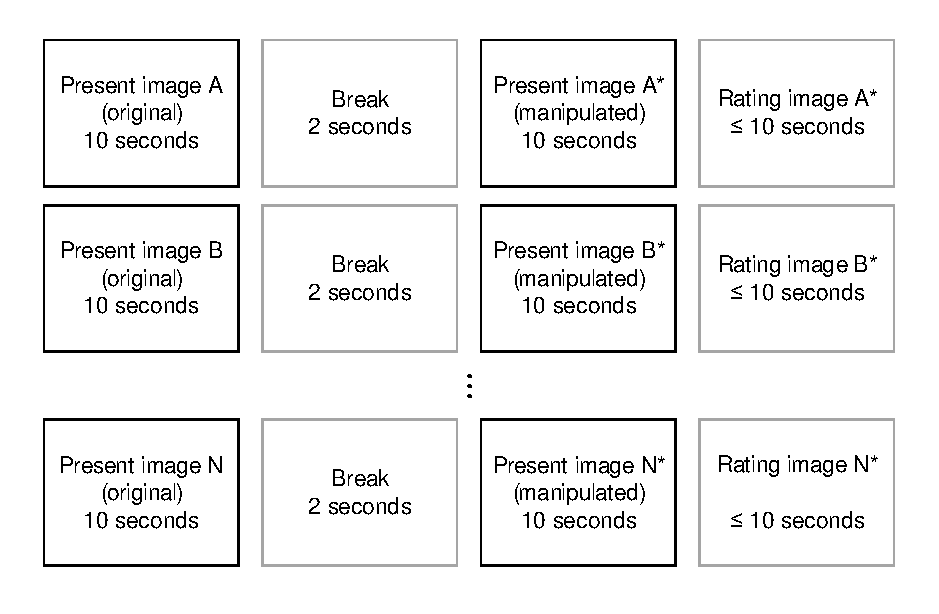
\includegraphics[width = 300pt]{Img/DCR.pdf}
	\caption{The process of the DCR assessment technique. Two stimulus are presented to the observer with a small break in between. The observer rates the second stimulus (modified) compared with the first stimulus (original).}
	\label{fig:dcrMethod}
\end{figure}

% section dcr (end)

\section{Subjective Assessment Methodology for Video \\Quality} % (fold)
\label{sec:samviq}

Subjective assessment methodology for video quality (SAMVIQ) is another assessment technique which differs from the other assessment techniques in multiple ways even though the labels; bad, poor, fair, good, and excellent are the same as the ones used in ACR. As the name says this technique is developed for use in video quality evaluation but the use of it for image quality evaluation is also seen \cite{Rouse2010}.

The rating scale in SAMVIQ differs hence it goes from 0 to 100 where the label 'bad' is aligned with the score 10 and the label 'excellent' is aligned with the score 90. This much larger scale has shown to be unnecessary large and the observers ratings might be grouped in 5 or 9 groups over the rating scale range \cite{Rouse2010}.

The process for the system also differs from earlier described systems. In SAMVIQ the process is split into a number of scenes where each scene contains a number of different variations of the same stimulus. Within a scene the observer can browse between the different variations of the stimulus. Also the observer is able to evaluate the image while observing it. When all stimulus has been rated another scene might be presented and the process repeats itself. Notice that the order of the different variations of a stimulus changes for every scene. The process is illustrated in \autoref{fig:samviqMethod}.

\begin{figure}[H]
	\centering
	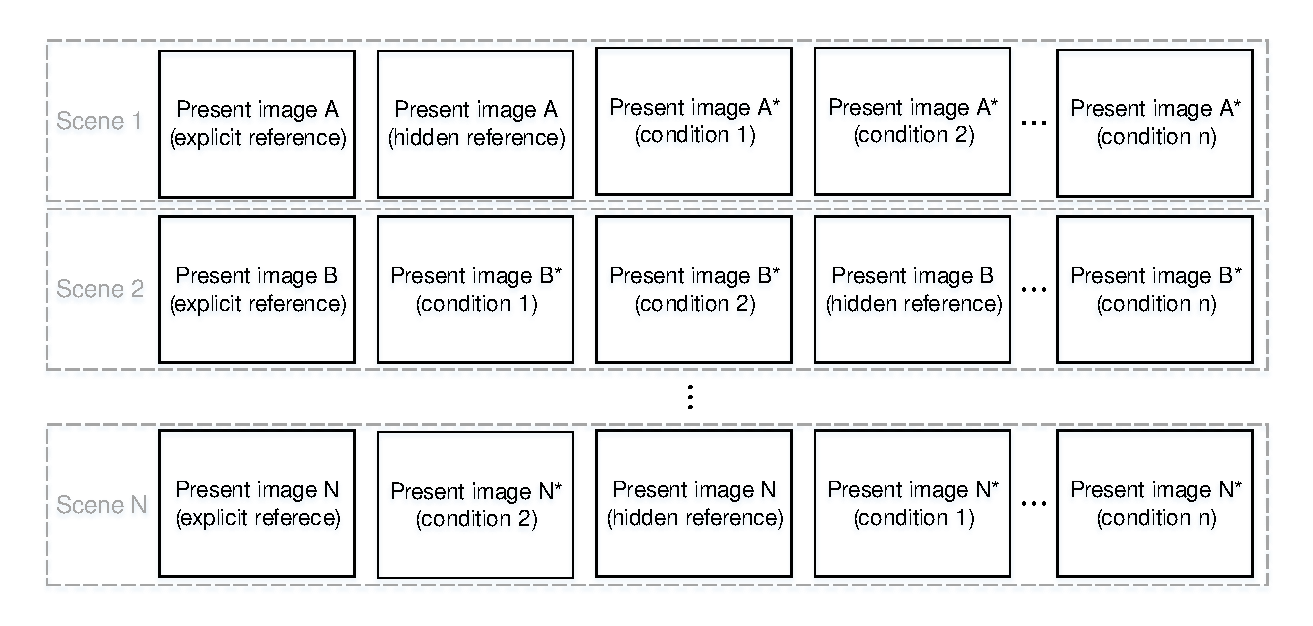
\includegraphics[width = \columnwidth]{Img/SAMVIQ.pdf}
	\caption{SAMVIQ method}
	\label{fig:samviqMethod}
\end{figure}

The illustration in \autoref{fig:samviqMethod} shows the use of a hidden reference. In SAMVIQ the use of a hidden reference is mandatory \cite{Kozamernik2005}.

% section samviq (end)

\section{Discussion} % (fold)
\label{sec:discussion}

The right choice of assessment technique depends highly on the application which it is used for. In this project it should be used to evaluations of images which lack of quality is imposed by some kind of lossy compression technique. The image quality will differ in range of very good quality to very poor quality. The evaluation assessment technique therefore must work for both cases. The hardest thing to evaluate is the smaller errors which can not be easily seen with the eye. Therefore the greatest constraint for the assessment technique is that it should give the observer the best opportunity to see and evaluate these type of errors.

The greatest benefit of the ACR method is that it is easy ti understand and implement. The drawback with respect to this project is that the ACR does not have an explicit reference which is recommended in evaluations when the impairments of the images are small \cite{ITU-TRecommendationP.9102008}. Both DCR and SAMVIQ has the ability of using an explicit reference.

One difference of DCR and SAMVIQ is the rating scale.As mentioned before experiments show that the rather large rating scale in SAMVIQ is superfluous \cite{Rouse2010} and the 5, 9 or 11 grade rating scale in DCR would be enough. 

Another difference of DCR and SAMVIQ is the 

Samviq muliggør/er oplagt for evaluering af samme billede under flere forskellige forhold. DCR lægger op til at det er forskellige 

% section discussion (end)